% It is an example file showing how to use the 'acm_proc_article-sp.cls' V3.2SP
% LaTeX2e document class file for Conference Proceedings submissions.
\documentclass{article}

\usepackage[letterpaper,breaklinks=true]{hyperref}
\usepackage{float}
\usepackage{graphicx}
\usepackage{indentfirst}
\usepackage{url}
\usepackage{listings}
\usepackage{xcolor}
\usepackage[none]{hyphenat}

% Macro for Bold Text
\newcommand{\Bold}[1]{\textbf{#1}}
\newcommand{\Italics}[1]{\textit{#1}}

\newcommand{\ClassName}[1]{\texttt{#1}}
\newcommand{\FunctionName}[1]{\textit{#1}}
\newcommand{\Code}[1]{\texttt{#1}}

\lstset { %
    language=C++,
    backgroundcolor=\color{black!5}, % set backgroundcolor
    basicstyle=\footnotesize,% basic font setting
}

% Metadata Information

\begin{document}

\markboth{Z. Jagannatha}{An Object-Oriented Circuit Simulation Library}

\title{An Object-Oriented Circuit Simulation Library}
\author{Zeal Jagannatha}

\maketitle

\begin{abstract}

The study of often digital electronics is introduced with the help of graphical tools. However, relatively little attention is given to code-based approaches. The C++ Circuit Simulation Library (CCSL), provides a C++ class library for working with simulated digital circuits, and gives users an efficient framework for digital circuit design and development.

\end{abstract}

\section{Introduction}

CCSL provides digital logic simulation facilities that can be used as a foundation for digital circuit development in C++. The library should be easily usable by users from a variety of experience levels from as simple as creating a pulse generator to as complicated as building an ALU. In addition, CCSL seeks to represent the interactions of real digital circuits as closely as possible. To this purpose, the projects provides functionality to simulate circuit creation, connection and evaluation with evaluators and circuit bread-boxes. In addition, tools are included that allow easy generalization of circuits, such as black-box components.

When pieced together correctly, basic components allow us to reach higher-level abstractions and focus on the functionality of collections of these components, rather than individual components. These collections are the typical focus of digital electronics within computer science. I.e. computer scientists ignore the resistors, capacitors and other details, and focus purely on the devices that can be made , e.g. \Bold{and}, \Bold{or}, and \Bold{not} gates.

CCSL users are assumed to have a basic familiarity with C++ programming. Users wishing to use the library to design new digital components must have an understanding of C++ inheritance [Stroustrup 2000]. Finally, in order to fully make use of all aspects of the project, an understanding of algorithms and data structures is necessary. In addition, hash tables, graph algorithms, and garbage collection play large roles of the project, but are not required for designing circuits or components of any kind.

\subsection{Notation}

In the remainder of this paper, words that are marked in \ClassName{typewriter font} are class names and always begin with a capital letter. Words that are in \FunctionName{Italics} are function names, and also begin with capital letters. Like class names, code samples are also in typewriter font, but do not begin with a capital letter.

\subsection{Intended Audience}

The intended audience of the project is programmers who wish to design and simulate digital circuits in C++. However, the user's level of experience limits the functionalities within the project that are accessible to them. From the point of view of the project, there are three experience levels that have different methods of interacting with the project: introductory users, advanced users, and expert users.

Introductory users are those who are able to create and use simple circuits assembled from pre-defined components. This group of users has little to no understanding of the traversal methods and design principles used within the library. This group of users would include students in introductory computer architecture or hardware courses.

Advanced users are those who additionally wish to create their own components by either extending existing components or by creating brand new components from scratch. These users can also extend the existing evaluation methods to their own uses. Such users have a good understanding of the principles used in the design of the project and can use this knowledge to extend their components and iterators. These users would be students who have completed courses in algorithms, object-oriented design, and computer hardware.

Expert users are users who are able to construct circuits from components, both predefined and of their own making, can extend existing iterators to create new ways of evaluating and interacting with circuits, and can freely modify the structure of the library to suit their needs. These users are those who understand not only the principles which the project was designed with, but have a good understanding of the internal mechanisms of the project as well.

\subsection{Related Work}

A variety of related projects have been produced:

\begin{itemize}

\item Logisim: A graphical circuit simulator. The project was thorough and implemented many of the features which CCSL implemented including breadth-first evaluation and black-box components [Burch 2002].

\item KLogic: A graphical circuit simulator. KLogic allows black-box components [Rostin 2001].

\item Verilog: A professional-level hardware description language that can be used to construct detailed models of digital circuits, down to the level of integrated circuit organization [IEEE 2006].

\item LibLCS: A code-based library for digital circuit simulation [Chandra 2007].

\end{itemize}

\section{Project Design}

\subsection{Example}

As a simple example, consider the design of a simple 2-to-1 Multiplexer:

\begin{figure}[H]
    \begin{center}
        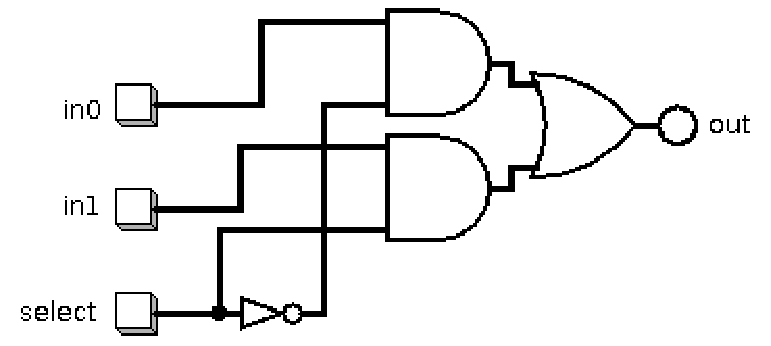
\includegraphics[angle=0,width=200pt]{imgs/Mux.pdf}
    \end{center}
    \caption{Circuit diagram for a 2-to-1 Multiplexer.}
\end{figure}

When designing the library, we would like the interface to be as intuitive as possible, and for a simple circuit to have simple code. This is the case for the 2-to-1 Multiplexer, as is the case with most components. The code for the Multiplexer is given below:

\begin{lstlisting}
// Create the Circuit Breadboard
Circuit topLevel;

// Declare Components
topLevel.AddComponent("Select", new Button());
topLevel.AddComponent("In0", new Button());
topLevel.AddComponent("In1", new Button());
topLevel.AddComponent("Out", new LED());
topLevel.AddComponent("Split", new Splitter(2));
topLevel.AddComponent("And0", new And());
topLevel.AddComponent("And1", new And());
topLevel.AddComponent("Not", new Not());
topLevel.AddComponent("Or", new Or());

// Connect the Components
topLevel.Connect("Select",0,"Split",0);
topLevel.Connect("Split",0,"And0",0);
topLevel.Connect("Split",1,"And1",0);
topLevel.Connect("In0",0,"And0",1);
topLevel.Connect("In1",0,"And1",1);
topLevel.Connect("And0",0,"Or",0);
topLevel.Connect("And1",0,"Or",1);
topLevel.Connect("Or",0,"Out",0);

// Specify the input and output components
topLevel.AddInput("Select");
topLevel.AddInput("In0");
topLevel.AddInput("In1");
topLevel.AddOutput("Out");

// Evaluate the Circuit
topLevel.Evaluate();
\end{lstlisting}

The meaning of the specific function calls will be explained later, but the general idea when trying to convert a circuit to its cooresponding code there are a few steps that must be taken. First, the user must declare components, then they must be connected with wires. Once the user has done this, they must specify the inputs and outputs to the circuit, and trigger the evaluation.

From that point on, the circuit will evaluate itself and return control back to the user, allowing them to view the resulting values. All of this interaction can be done through the use of a \ClassName{Circuit}, in this example called \ClassName{topLevel}. This common interface and other features have been provided to make code generation with this library as simple and easy as possible.

\subsection{Organization}

The organizing concept for the project is that of a breadboard into which a user plugs components. This model is general and intuitive. In addition, certain methods can be used by the implementation of the breadboard to make accessing and using components easier. For example, component connection can be done without any direct contact with wires.

\subsection{Evaluation Model}

Digital components are thought of as being akin to programming language functions. Similarly, wires are akin to simple values. Evaluating a circuit would conceptually produce a series of function calls passing along different values which can be simulated with function composition. However, while this view of circuits is sufficient to model combinational circuits, it is inadequate to model sequential circuits. Sequential circuits would not work because they are circuits that contain feedback, or loops. Naively implemented, this method would cause the simulator to enter an infinite loop when simulating sequential circuits via function composition.

However, this view of things is not without merit. In particular, it provides a simple way of conceptualizing the interaction between components and wires that expands with some work to sequential circuits; components are function-like things that perform operations on wires, which store the states of the circuit. This is the method for interaction between wires and components that the library is based on.

The other main aspect of component interaction is the evaluation method. There are two main ways of approaching this problem. The first, and simpler approach, is to treat the components as vertices in a graph with the wires designating edges. This leads us to two main ways of evaluating the circuit, based on graph traversal techniques. Depth-first traversal is generally unhelpful for simulating circuits, so we use breadth-first traversal to evaluate the components. This gives us the first method for circuit traversal. This method proves to have significant differences with the behavior of actual circuits, however.

In actual digital circuits, each component has an inherent delay that it introduces before it propagates its results to further components. This delay is ignored by the depth-first traversal method, but in order to fully simulate the behavior of real digital circuits, we cannot ignore this propagation delay. The second method is an order that takes delays into account and evaluates the components in an order equivalent to evaluating actual digital components.

\subsection{Idioms and Design Patterns}

The design and implementation of the library uses several programming idioms and design patterns [Gamma 1995] to simplify and generalize the layout of the project:

\subsubsection{Iterator}

To generalize the various ways in which a circuit can be evaluated or traversed, the project makes use of the iterator design pattern. This allows it to scalably implement evaluators for both traversal patterns as well as other iterators with other purposes. The iterator pattern is used by creating a class heirarchy that provides a variety of methods for circuit evaluation with a single interface enforced by inheritance.

\subsubsection{Observer}

For simulating probes and detecting uncontrolled feedback loops, the observer design pattern is used. The Observer pattern is used by designing wires to inherit from an Observer base class, which allows a user to attach probes to the wires to observe their state.

\subsubsection{Handle-Body}

In order to present a clean interface to users, the project uses the handle-body idiom to generalize circuit components and allow the interface to be pointer-free, which increases its readability.

\subsection{Infinite Oscillation}

When simulating sequential circuits, there is the problem of detecting loops that never stabilize. In general, deciding if a particular circuit has a set of input states that create an infinite oscillation when evaluated is believed to be NP-complete [Cormen 2009]. As a result, a simple strategy is applied that works well in most, but not all, cases. This heuristic is to keep track of how many times each wire’s state has been changed. If a wire's update count exceeds a pre-defined amount, we assume that the circuit has entered an infinite loop and cease evaluation of the circuit.

\section{Implementation Details}

\subsection{Library Structure}

The class sturcture is divided into several main modules. In programming, these modules take the form of class heirarchies. In source code, the various files are organized into the following folders:

\subsubsection{BaseCircuits}

Contains definitions for the built-in components. These built-in components include components for basic logic, input/output, flip flops and latches, and simple arithmetic.

\subsubsection{Circuit}

Contains the class files for the \ClassName{Circuit} class, which implements a breadboard circuit. Components can be added to the circuit with the addition of an identifier, or string name. This allows them to be referenced by this identifier, eliminating the need to explicitly reference the component and alloing more helpful error messages. The \ClassName{Circuit} class makes use of a hash table to efficiently store these components by name, provided by the sparsehash library, which is mentioned below.

\subsubsection{CircuitEvaluator}

Contains the definitions for the Evaluator classes. Evaluators for debugging, normal (BFS) evaluation, and delay-based evaluation are included.

\subsubsection{CircuitIterator}

Contains the definitions for the two Iterators, \ClassName{BFSIterator} and \ClassName{DelayCircuitIterator}. The former is used to model breadth first iteration, and latter is used to simulate component delays.

\subsubsection{Component}

Contains the definitions for the component classes. This is the most pivotal part of the project as most of the other classes are groundwork or wrappers for this class. The handle-body idiom is used to allow pointer-less interaction with Component class instances. The handle is named \ClassName{Component} and the body is named \ClassName{CustomComponent}.

\subsubsection{Exceptions}

Contains the definitions for the Exceptions used in the project. This includes exceptions for circuit evaluation errors, component errors, and wire errors.

\subsubsection{Observer}

Implementation of the Observer design pattern. Also contains the implementation of probes which can be attached to wires to view their state.

\subsubsection{Wire}

Defines the interface for wires. Primarily this is used internally, and users will nearly never interact with these directly.

\subsubsection{gc}

Implementation of the Conservative Garbage Collector, which is used to include garbage collection in the project [Boehm 1993].

\subsubsection{sparsehash}

Implementation of the Sparse Hash Library, which is used to include hash tables in the project [Silverstein 2012].

\subsection{Wire States}

The wire states for the project are implemented as an ordered pair $(t,s)$ where $t$ is the timestamp the wire was last updated, and $s$ is the state it was given at that time. This allows the evaluator to keep track not only of the states being passed along wires, but also the time delay introduced by components in the circuit. The primary class for this implementation is the \ClassName{State} class, which includes the timestamp, state pair.

The timestamps passed around are implemented as quads (64-bit integers) to allow for very large timestamps for larger circuits that take much longer to run. In addition, the unit for these timestamps is defined as the amount of time it takes a negation component to operate. This unit is chosen since it is the smallest and simplest component that does some form of computation, unlike a splitter, for example, which simply passes its value along to its outputs, and does not introduce any delay.

\subsection{Component Classes}

Certain pre-defined components have been provided. These components include both simple logical components that are required for building more advanced circuits, as well as more complicated components that have been provided to demonstrate certain aspects of the project's implementation or design.

\subsubsection{Combinatorial Components}

The predefined logic components primarily include basic logic components, but also include components necessary for the organization of circuits:

\begin{itemize}

\item Unary \ClassName{Not} gate.

\item Binary \ClassName{And} gate.

\item Binary \ClassName{Or} gate.

\item Binary \ClassName{Nor} gate.

\item Binary \ClassName{Xor} gate.

\item A \ClassName{Splitter} propagates a single value to several components.

\item \ClassName{Ground} is the ground of the circuit, and accepts inputs, without providing any outputs.

\end{itemize}

\subsubsection{Input/Output Components}

Input and output to circuits and components is done with instances of the \ClassName{CircuitInput} and \ClassName{CircuitOutput} classes. These two classes provide a generalized interface for interacting with circuits via their input and output components. From these two generalized interfaces, more specific classes have been derived. For input, the components are:

\begin{itemize}

\item A \ClassName{Button} allows circuit input from standard input.

\item The \ClassName{StreamInput} device is like a \ClassName{Button}, but reads from an arbitrary input steam.

\item A \ClassName{Toggle} is a device that is toggled on and off, rather than assigned a specific state.

\end{itemize}

For output, the predefined components are:

\begin{itemize}

\item An \ClassName{LED} functions by displaying a value on the standard output device.

\item A \ClassName{StreamOutput} is like an LED but displays to an arbitrary output steam.

\end{itemize}

Besides these, components have been provided for input and output to and from busses: \ClassName{BitVectorInput} and \ClassName{BitVectorOutput}.

\subsubsection{Advanced Components}

In addition to the above components, more advanced components have been created to demonstrate other capabilities of the system. These include:

\begin{itemize}

\item A 1-bit \ClassName{FullAdder}, which demonstrates basic arithmetic.

\item An \ClassName{SRlatch} and \ClassName{JKflipflop} which demonstrate the use of sequential components.

\end{itemize}

\subsubsection{Black-box Components}

In addition to providing pre-defined components, CCSL permits users to define their own components. To this purpose, black-box components have been included. This interface allows users to create components from circuits they have already built, which can then be used in other circuits. The class \ClassName{BlackBox} implements these features. In order to use this class, a user need only define a class with whatever name they would like to give their component, inherit from \ClassName{BlackBox}, provide the \FunctionName{Delay} function, and within the constructor create the circuit as they would within the main function of a circuit, using the result of the \FunctionName{Internal} function as the top-level circuit. As an example of this, the pre-defined \ClassName{JKflipflop} component has been created in this way. The source code for this class is below.

\begin{lstlisting}
class JKflipflop : public BlackBox {

protected:

    // Returns the delay of the component
    State::Timestamp Delay() {
        return 10;
    }

public:

    // Constructor
    JKflipflop()
        // A JK flipflop is a BlackBox with 2 inputs and 2 outputs
        : BlackBox("JKflipflop", 2, 2)
        {

        // Build the black box's subcircuit within the constructor.

        internal().Link("J", new CircuitInput());
        internal().Link("K", new CircuitInput());
        internal().Link("AndJ", new And());
        internal().Link("AndK", new And());
        internal().Link("SR", new SRlatch());
        internal().Link("Qsplit", new Splitter(2));
        internal().Link("qsplit", new Splitter(2));

        internal().Link("Q", new CircuitOutput());
        internal().Link("q", new CircuitOutput());

        internal().LinkInput("J"); // Input 0
        internal().LinkInput("K"); // Input 1
        internal().LinkOutput("Q"); // Output 0
        internal().LinkOutput("q"); // Output 1

        internal().LinkWithWire("J", 0, "AndJ", 0);
        internal().LinkWithWire("K", 0, "AndK", 0);
        internal().LinkWithWire("AndJ", 0, "SR", 0);
        internal().LinkWithWire("AndK", 0, "SR", 1);
        internal().LinkWithWire("SR", 0, "Qsplit", 0, false);
        internal().LinkWithWire("SR", 1, "qsplit", 0, true);
        internal().LinkWithWire("Qsplit", 0, "Q", 0, false);
        internal().LinkWithWire("qsplit", 0, "q", 0, true);
        internal().LinkWithWire("Qsplit", 1, "AndJ", 1, false);
        internal().LinkWithWire("qsplit", 1, "AndK", 1, true);
    }
};
\end{lstlisting}

\subsection{Class Interaction}

The project's classes interact in a variety of ways. The goals for such interaction can be adding a component to a circuit breadboard, querying the state of a component, evaluating a circuit, and other operations on circuits. For these operations, the interaction is fairly simple. What follows is a description of the various interaction mechanisms.

\subsubsection{Component Construction}

Component creation is also done via the \ClassName{Circuit} class. This allows \ClassName{Circuit} to be a single interface for all the necessaries of component interaction.

The diagram below demonstrates the interactions between the user (far left), \ClassName{Circuit}, and hash table. Before a \ClassName{Circuit} can be used, it must be created. This can be done by the use of its default constructor indicated by section \Bold{A} in the figure below. No additional work is needed to create the circuit, as the constructor does all the necessary setup. For creating a component, the \ClassName{Circuit} class provides the \FunctionName{AddComponent} function, which adds a component to the Circuit with a particular name; represented by section \Bold{B} on the figure below. The \FunctionName{AddComponent} function requires a \ClassName{Component}, passed by pointer, and a string for the name. The \ClassName{Component} is generally passed by using \ClassName{new Component}, since it is garbage collected. The string has no restrictions except that each component’s name must be unique in a given \ClassName{Circuit}. For accessing that component later, the function \FunctionName{Lookup} is
provided, which looks a component up by name; represented by section \Bold{C} in the figure.

\begin{figure}[H]
    \begin{center}
        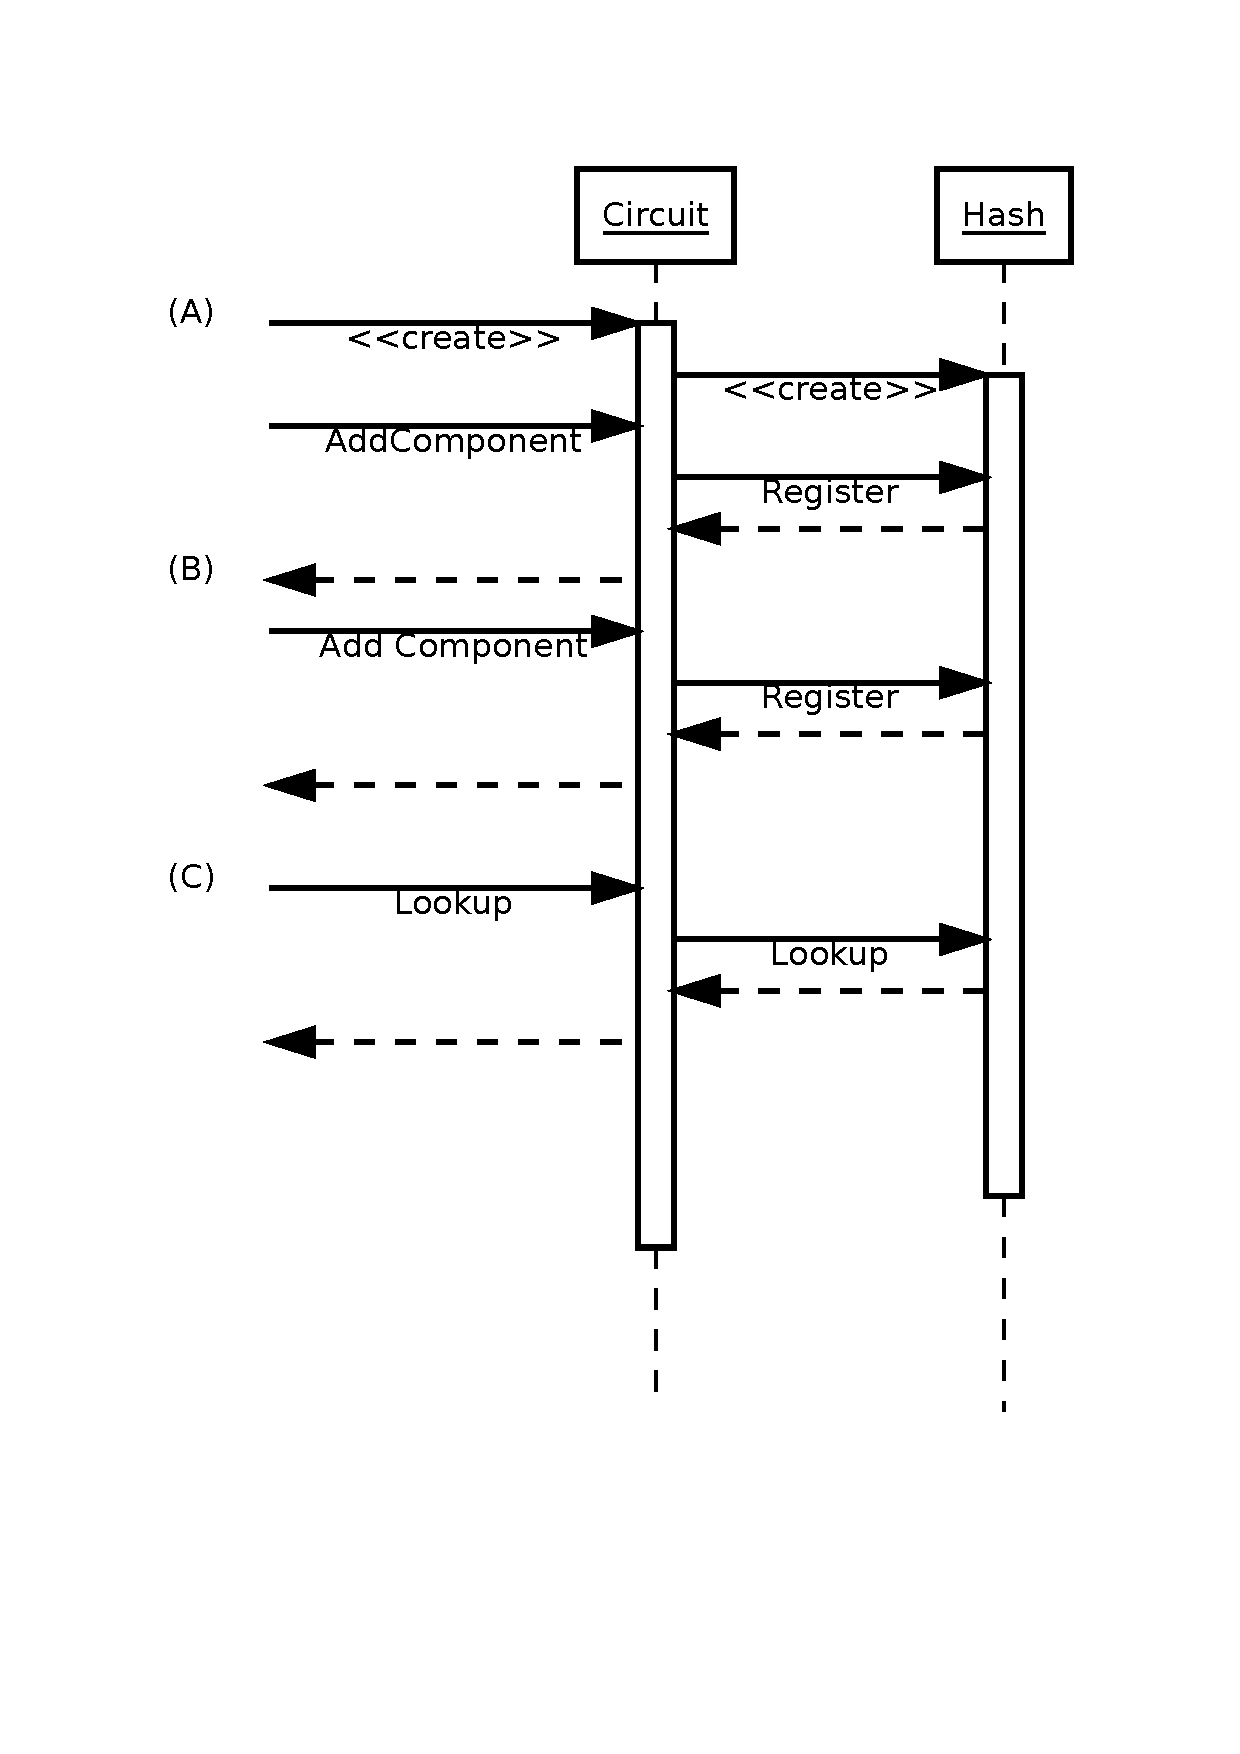
\includegraphics[angle=270,width=200pt]{imgs/ComponentCreationInteraction.pdf}
    \end{center}
    \caption{Interactions between a \ClassName{Circuit} and hash table when creating components.}
\end{figure}

The following code fragment exemplifies the syntax for component creation:

\begin{lstlisting}
// Create the circuit
Circuit topLevel;

// Create the components:

// Add a component called "in" that is a button.
topLevel.AddComponent("in", new Button());

// Add a component called "out" that is an LED.
topLevel.AddComponent("out", new LED());
\end{lstlisting}

\subsubsection{Component Connection}

To create and evaluate circuits is important, but means nothing without the ability to connect components. This allows the user to specify the way in which the components interact. Like component creation and evaluation, connection is done with the \ClassName{Circuit} class. The class provides the member function \FunctionName{Connect}, which takes four parameters: the input component, the input pin number, the output component and the output pin number. This function creates a \ClassName{Wire} and associates the wire's input with the specified pin number of the input component, and the wire's output with the specified pin number of the output component. The diagram below demonstrates the interaction between a \ClassName{Circuit} and the newly created \ClassName{Wire}.

\begin{figure}[H]
    \begin{center}
        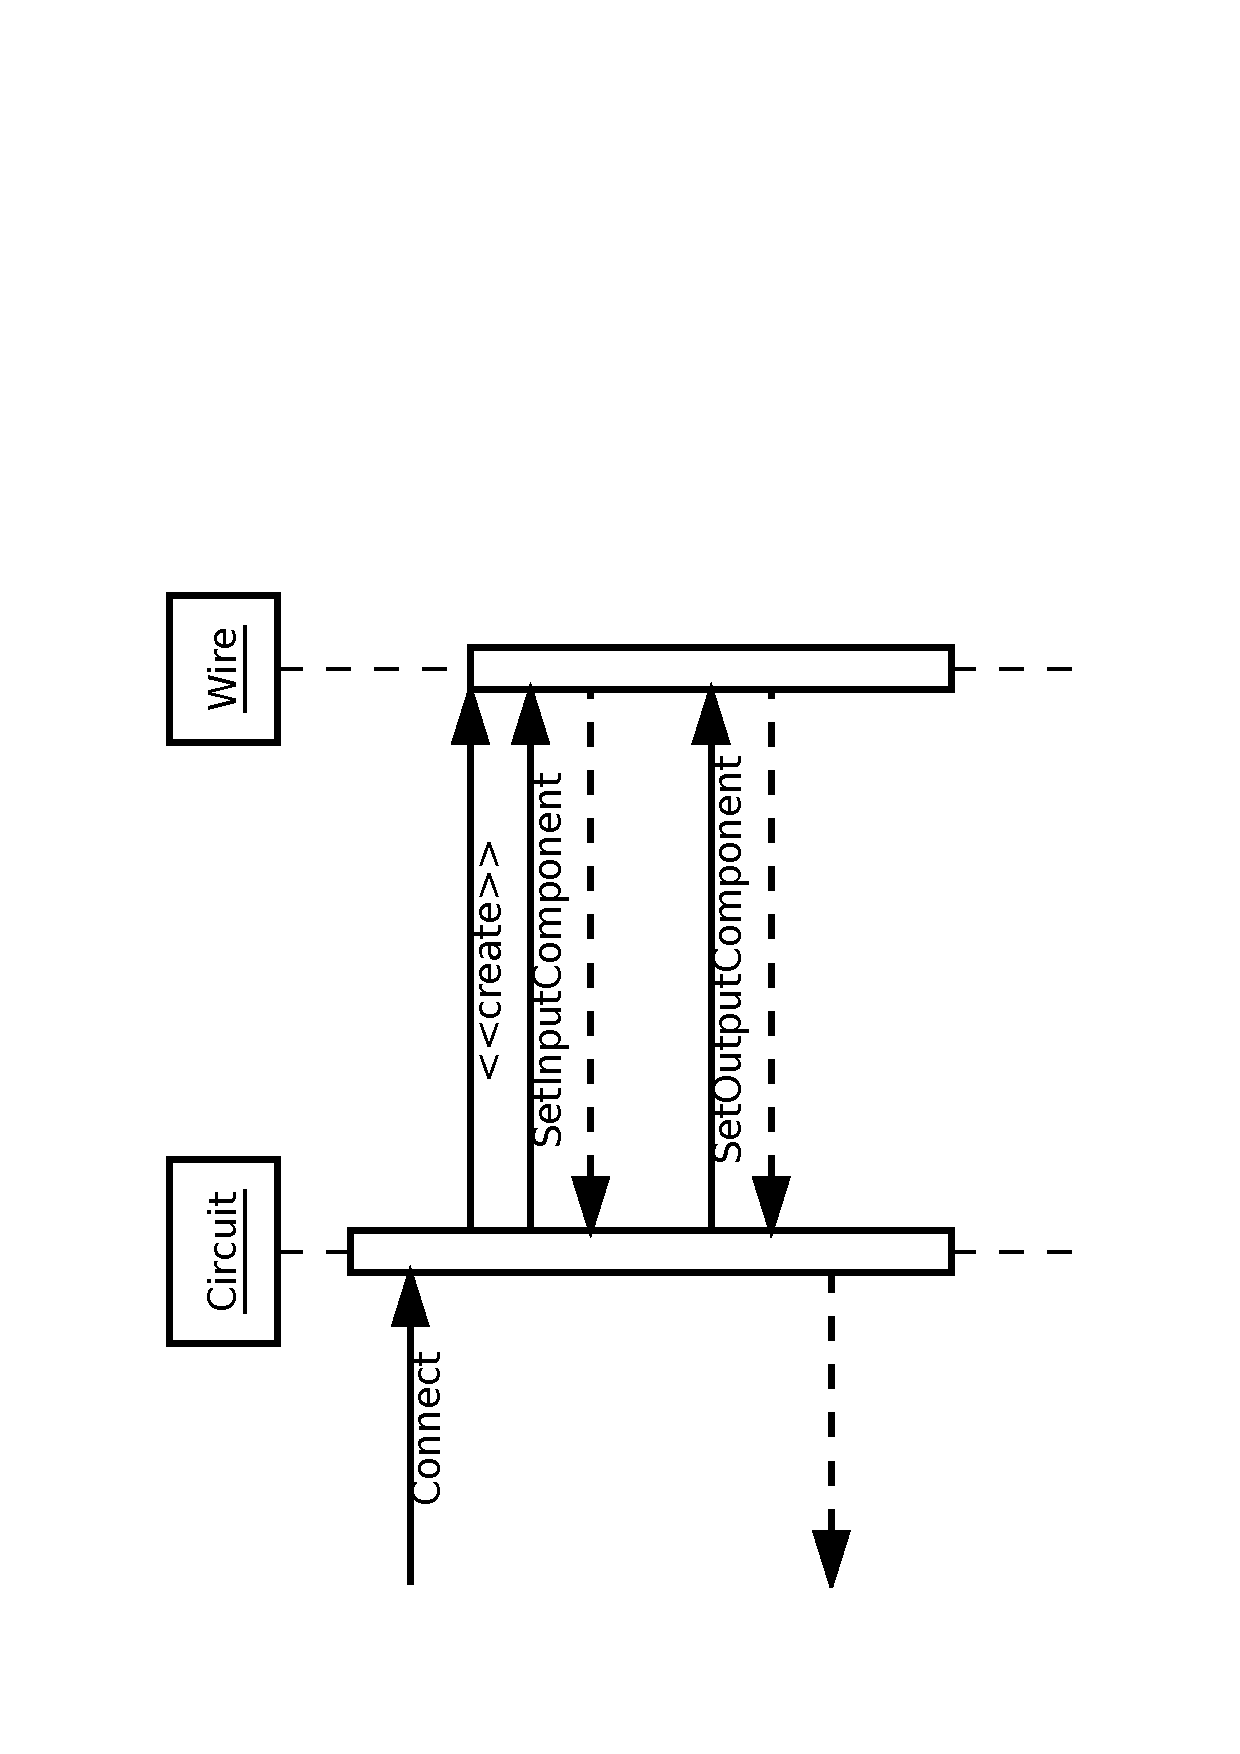
\includegraphics[angle=270,width=200pt]{imgs/ComponentConnectionInteraction.pdf}
    \end{center}
    \caption{Interactions between a \ClassName{Circuit} and \ClassName{Wire} when connecting components.}
\end{figure}

The following code fragment provides an example of the syntax for component connection:

\begin{lstlisting}
// Using topLevel from the previous  code sample:

topLevel.Connect("in",0,"out",0);
\end{lstlisting}

\subsubsection{Circuit Evaluation}

Perhaps the most important mechanism for a single run of a circuit is the evaluation of the components. To fully simulate the interactions for circuit evaluation, the project includes the \ClassName{CircuitIterator} class hierarchy. This class is the base class for all classes that implement evaluation of a circuit.  An abstract base class is used to allow users to define their own evaluators that extend or alter pre-defined evaluation techniques. Three pre-defined circuit evaluators have been provided that allow different ways of modeling circuit interaction, \ClassName{NormalEvaluator} which implements BFS evaluation, \ClassName{DelayEvaluator} which implements delay-based evaluation, and \ClassName{Debugger}
 which allows a user to interact with the circuit as a delay-based evaluation takes place. These evaluators are discussed in more detail below.

The interaction between the classes themselves is fairly simple. Upon a call to a circuit's evaluate function, the circuit creates an evaluator that matches with the circuit’s evaluation method and then uses this evaluator to evaluate the components within itself. An sequence diagram of this interaction is used below to detail class interactions. This diagrams shows the function calls and returns across classes with arrows. Each solid arrow represents a function call from one class to another. Dotted arrows represent function return from previous calls. In each diagram, there is an implicit user on the far left, making the left-most calls through either a main function, or within a black-box component.

\begin{figure}[H]
    \begin{center}
        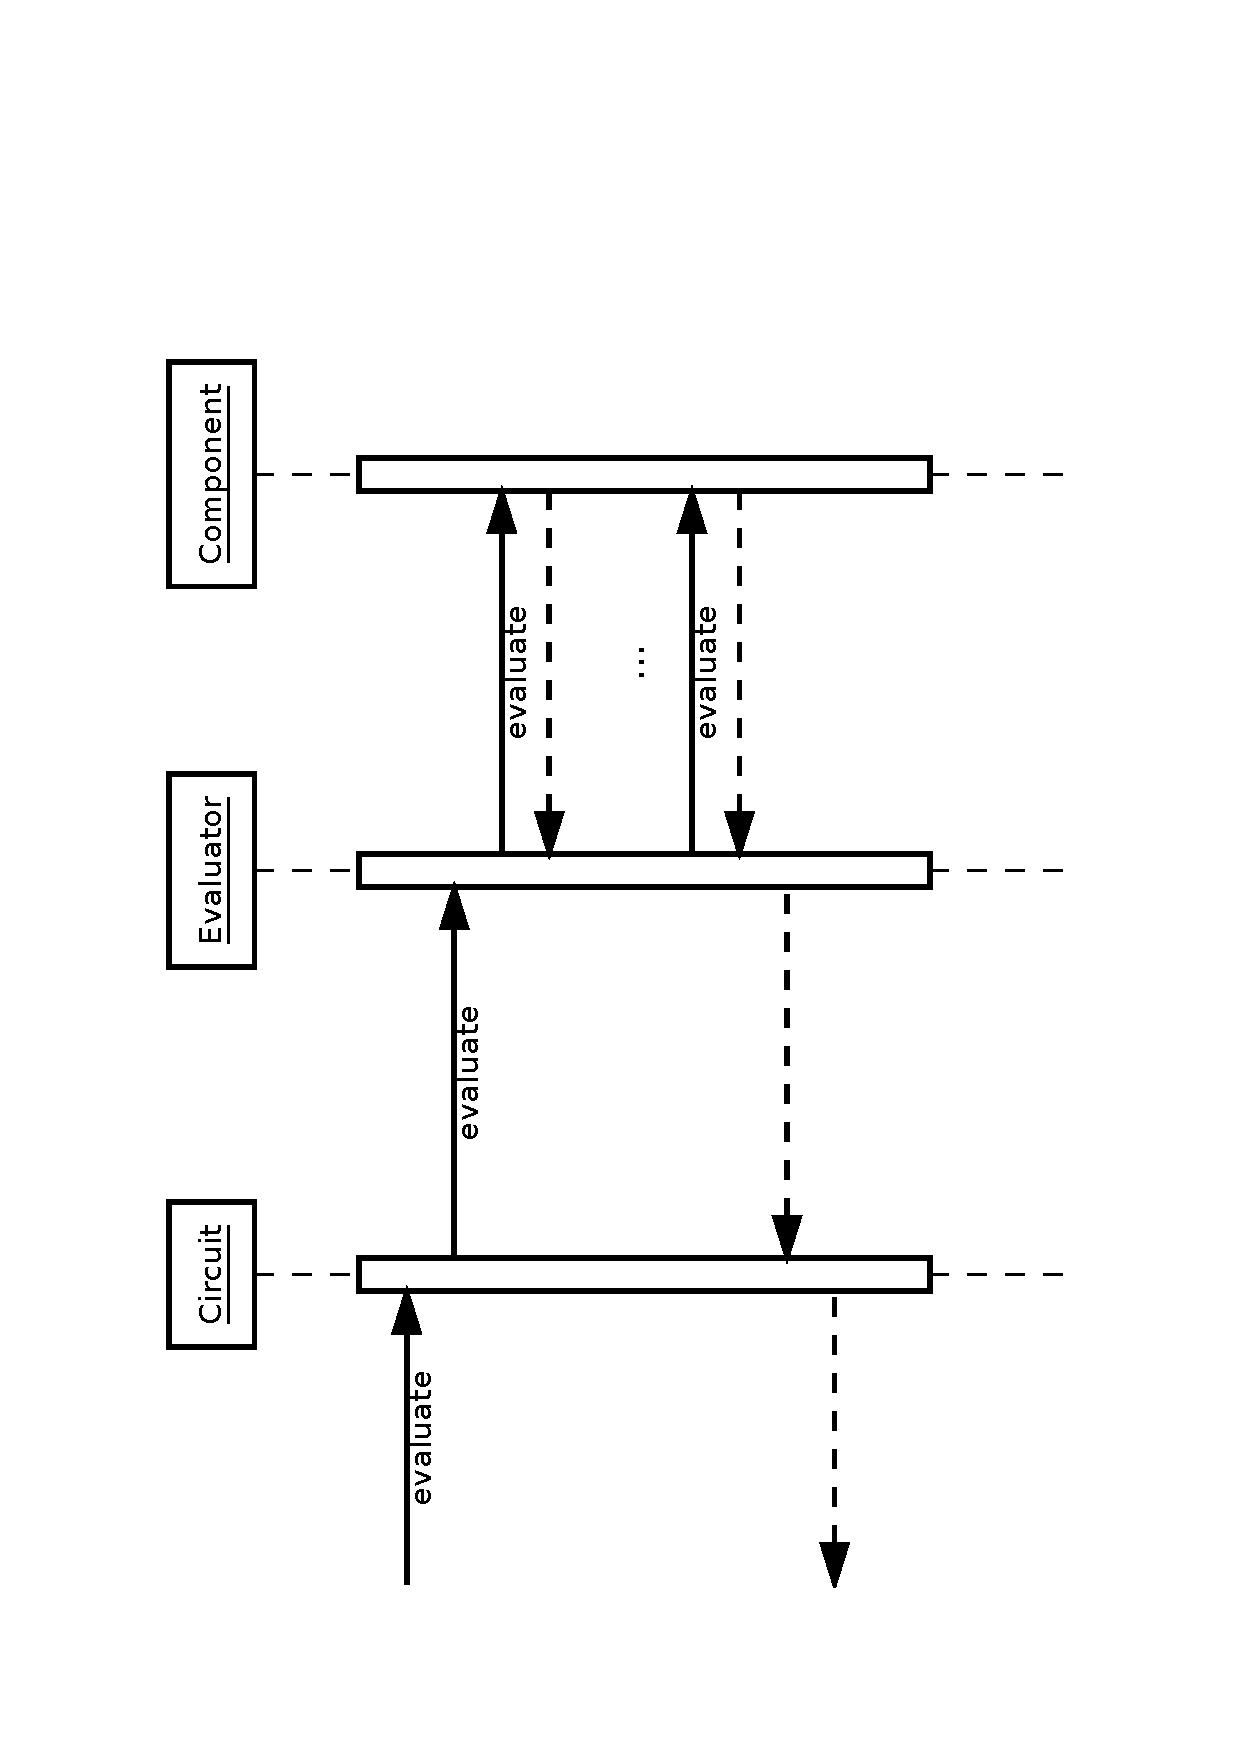
\includegraphics[angle=270,width=200pt]{imgs/CircuitEvaluationInteraction.pdf}
    \end{center}
    \caption{Interactions between the circuit, evaluator, and components when evaluating a circuit.}
\end{figure}

Circuit evaluation is done by classes derived from which is based on the \ClassName{CircuitIterator} class. This \ClassName{CircuitIterator} ensures that the evaluators share a similar interface, but provides few restrictions on their behavior. As a result of this, evaluators can choose any order in which to evaluate components. In addition, there is nothing preventing components from being evaluated more than once, or not at all, in fact both these possiblities are used by some evaluation methods. In particular, all the built-in evaluators can evaluate components many times. Due to this lack of restriction, it is the responsibility of the evaluator to determine in which order the components are evaluated and keep track of them internally.

The two built-in evaluation techniques are breadth first evaluation and delay-based evaluation. Both of these methods are provided as a way of simulating real circuits, although each has their own advantages and disadvantages. Of the two, delay-based evaluation comes closer to the behavior of actual circuits, but breadth first evaluation has the advantage of being easy to understand from the point of view of the component interactions, as well as the implementation, since a plain queue can be used, rather than a priority queue.

A third implemented evaluator, the \ClassName{Debugger}, is based on a modified version of delay-based evaluation. A \ClassName{Debugger} evaluates a circuit using delay-based evaluation, but stops at each component to print diagnostic output, and prompt the user for input. This allows the user to see what is happening and interact with the circuit’s evaluation. Debugging is indicated for use when a \ClassName{Circuit}'s \FunctionName{Debug} function is called.

For a given circuit, the user can select which of these two evaluation methods are to be used by calling either of the functions \FunctionName{UseGateDelays} or \FunctionName{IgnoreGateDelays}, which enable or disable using gate delays, respectively. Alternatively, using a \ClassName{Debugger} to evaluate the circuit can be done by calling a circuit's \FunctionName{Debug} function.

The following example indicates all three types of evaluation methods.

\begin{lstlisting}
// Using topLevel from the previous  code sample:

// Desegnate the input and output components
topLevel.AddInput("in");
topLevel.AddOutput("out");

// The default behavior is delay-based evaluation.
// This can be changed with the function IgnoreGateDelays
topLevel.IgnoreGateDelays();

// Evaluate the circuit using breadth-first evaluation.
topLevel.Evaluate();

// The circuit can be changed back by using the function UseGateDelays
topLevel.UseGateDelays();

// Evaluate the circuit using delay-based evaluation.
topLevel.Evaluate();

// The circuit can be debugged by using the function Debug
// which evaluates the circuit using debugging.
topLevel.Debug();
\end{lstlisting}

Regardless of which type of evaluation the user selects, the evaluator needs to know which components indicate the components at which evaluation begins. This is done with the \FunctionName{AddInput} function, which allows the user to indicate which components should start the circuit’s evaluation.

\section{Future Work}

\subsection{Detecting Oscillation is NP-Complete}
A proof that detecting circuit oscillation is NP-complete has not been provided for this specific example. This proof would be a proof by reduction, as proofs of NP-completeness generally are. The outline of the proof is that detecting oscillation would require keeping track of every possible state in which the circuit has been. While finite, the number of possible states is likely to be exponential at worst-case, so such an algorithm would be at best exponential in space, which implies exponential in time.

\subsection{Circuit Iterators and Evaluators}
In addition, the concepts of circuit iterators and circuit evaluators aren't necessarily distinct at this time. If given more time, the two concepts could be made into disjoint but related ideas and that difference could be made more clear in code. In particular, iterators should be objects that iterate over components in a circuit without necessarily the goal of evaluating them, e.g. an iterator could be used to search over all components to find a particular component by name. On the other hand, evaluators would be designed with the specific purpose of evaluating a circuit. This would lead them to take either the delay-based or breadth-first approaches, as discussed above. For example, in addition to the three existing evaluators, one could be added that computes the delays for circuits, eliminating the need to define the \FunctionName{Delay} function in custom built components.

\subsection{Busses}
Finally, although busses were thought of as a desirable feature of the project, they were not a focus of the design. As a result, they can be made to work with for loops and similar ad-hoc techniques, but the approach doesn’t fit with the interface for most other interactions to the library. In the future, busses could be made to work by generalizing the concept of wires to wire groups or busses. This would allow users to link wire groups between components, rather than single wires. Changing the interaction in this way would still allow users to use single wires -- they would merely be interacting with unary wire groups - but allows simple interfaces for busses. If this change were made, it would be fairly easy to permit components to name ports, allowing users to reference them by name, rather than by an integer reference. This would greatly simplify construction of circuits such as SR-latches, where each input and output has a specific name, but arbitrary ordering.

\section{References}

[Boehm 1993] Boehm, H. 1993. Space efficient conservative garbage collection. ACM SIGPLAN.

[Burch 2002] Burch, C. 2002. Logisim: A graphical tool for logic circuit design and simulation. Journal of Educational and Resources in Computing.

[Chandra 2007] Chandra, S. 2007. libLCS: A logic circuit simulation library in C++. http://liblcs.sourceforge.net/

[Cormen et al. 2009] Cormen, T., Leiserson, C., Rivest, R., and Stein, C. 2009. Introduction to algorithms. The MIT Press.

[Gamma et al.1995] Gamma, E., Helm, R., Johnson, R., and Vlissides, J. 1995. Design patterns. Addison-Wesley.

[IEEE 2006] IEEE. 2006. Ieee standard for verilog hardware description language. Institute of Electrical and Electronics Engineers.

[Rostin 2001] Rostin, A. 2001. http://www.a-rostin.de/. Klogic: Digital circuit simulation.

[Stroustrup 2000] Stroustrup, B. 2000. The C++ Programming Language. Addison-Wesley.

[Silverstein 2012] Silverstein, C. sparsehash: An extremely memory-efficient hash\_map implementation. http://code.google.com/p/sparsehash/

\end{document}
